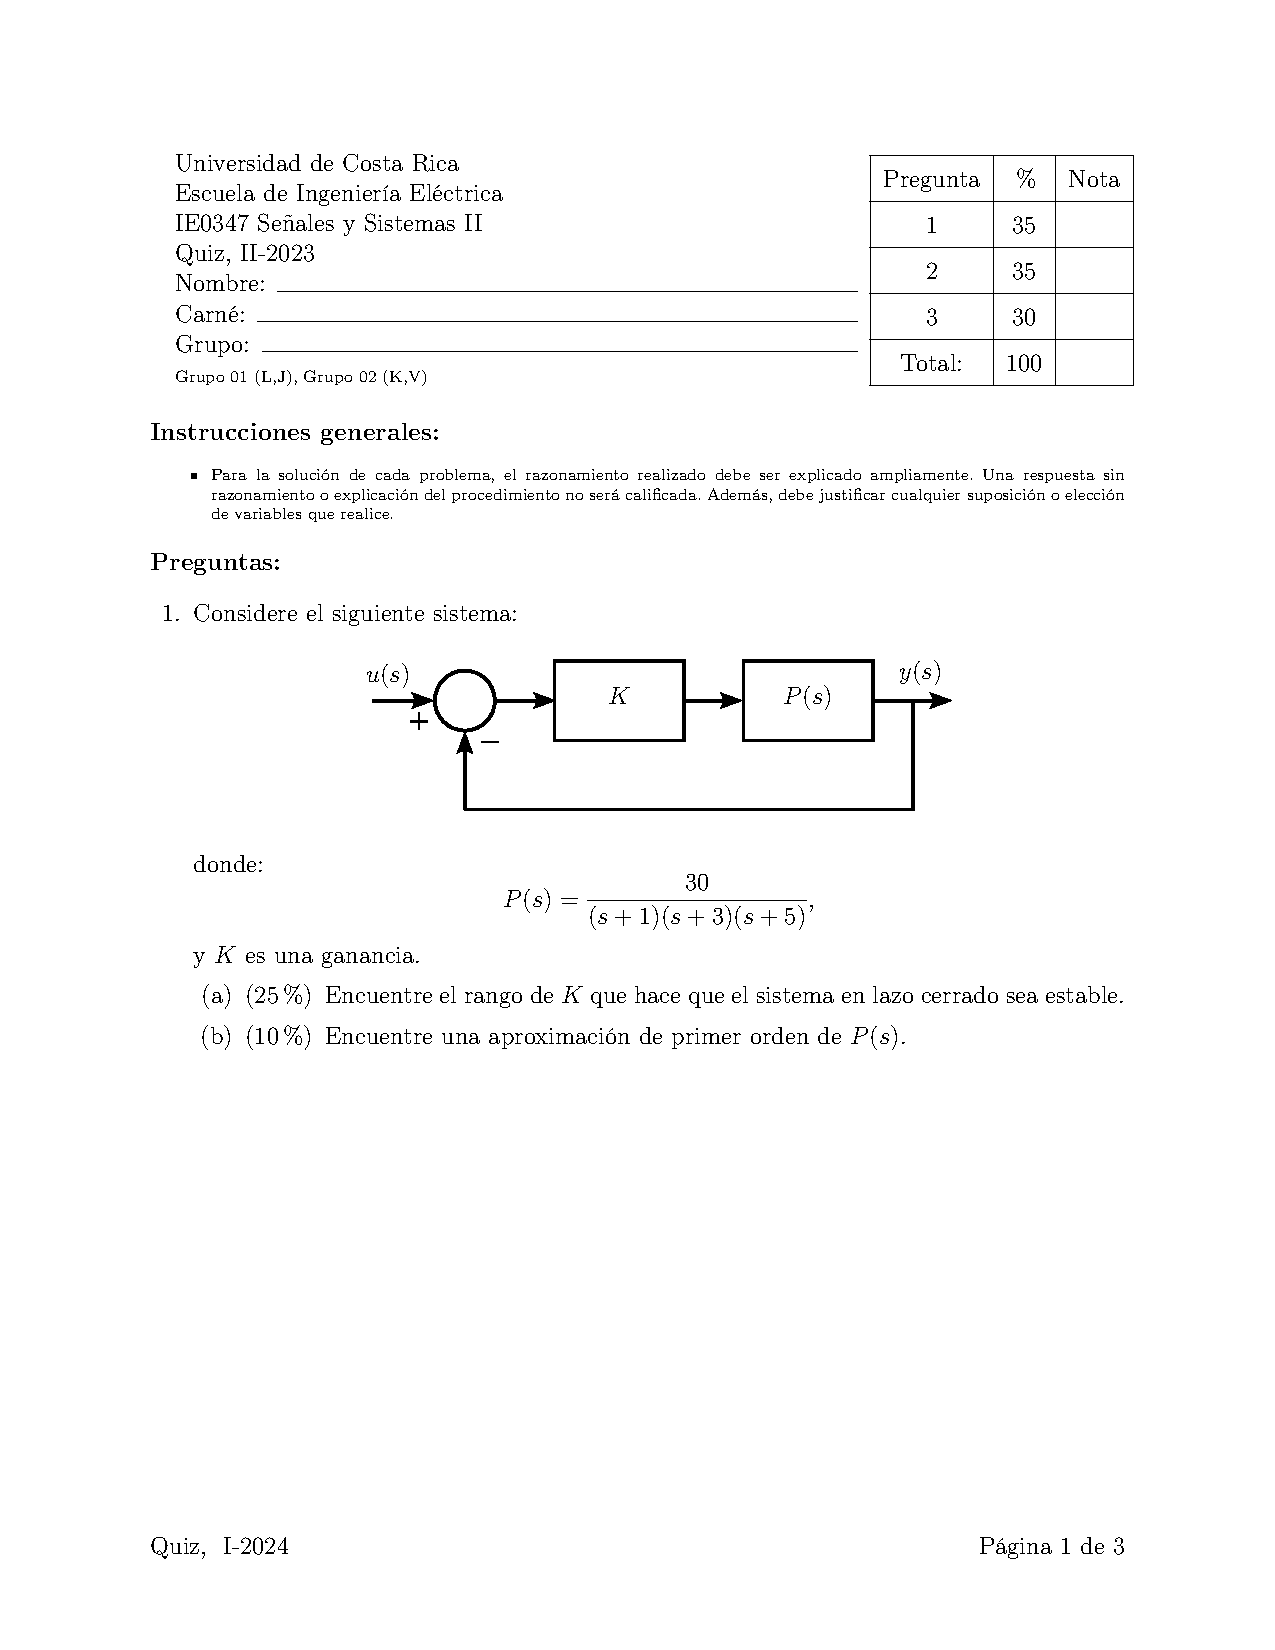
\includepdf[pages=1]{Quiz1.pdf}
\section{Solución 1}

\newcommand{\polinomio}{s^3+9s^2+23s+15}

Primero se combina en cascada ambos bloques \\

\begin{equation*}
    K \cdot P(s) = \dfrac{K \cdot 30}{\polinomio}
\end{equation*}

Después se realiza la eliminación del lazo de realimentación

\begin{equation*}
    H(s) = \dfrac{
    \dfrac{K \cdot 30}{\polinomio}
    }{
    1 + \dfrac{K \cdot 30}{\polinomio}
    }
\end{equation*}

Simplificamos

\begin{equation*}
    H(s) = \dfrac{
    \dfrac{K \cdot 30}{\polinomio}
    }{
    \dfrac{\polinomio}{\polinomio} + \dfrac{K \cdot 30}{\polinomio}
    }
\end{equation*}

\begin{equation*}
    H(s) = \dfrac{
    \dfrac{K \cdot 30}{\cancel{\polinomio}}
    }{
    \dfrac{K \cdot 30 + {\polinomio} }{\cancel{\polinomio}}
    }
    =
    \dfrac{K \cdot 30}{{\polinomio} + K \cdot 30}
\end{equation*}

\vspace{0.1cm}

La primera condición del criterio de estabilidad absoluta de Routh-Hurwitz
indica que los coeficientes del polinomio caracteristico deben ser todos del 
mismo signo, además la segunda condición indica que ningún coeficiente puede
ser cero por lo que:

\begin{equation*}
    K \cdot 30 + 15 > 0
\end{equation*}
\begin{equation*}
    K \cdot 30 > -15
\end{equation*}
\begin{equation*}
    K  > \dfrac{-1}{2}
\end{equation*}

\newpage

Se obtuvo la cota inferior del rango de estabilidad, por lo que ahora se 
procede a aplicar el arreglo de Routh-Hurwitz



\[
    \begin{array}
    {c|cc}
    s^3 & 1 & 23 \\
    s^2 & 9 & (15 + 30K) \\
    s^1 & a_{31} & a_{32} \\
    s^0 & a_{41} & a_{42} \\
    \end{array}
\]

\vspace{1cm}

\begin{equation*}
    a_{31} = \dfrac{207 - (15 + 30K) }{9} = \dfrac{64}{3} - \dfrac{10}{3} K
\end{equation*}

\vspace{0.1cm}

\begin{equation*}
    a_{32} = \dfrac{9 \cdot 0 - 1 \cdot 0}{9} = 0
\end{equation*}

\vspace{0.1cm}

\begin{equation*}
    a_{41} = \dfrac{(\dfrac{64}{3} - \dfrac{10}{3} K) \cdot (15 + 30K) - 9 
    \cdot 0}{\dfrac{64}{3} - \dfrac{10}{3} K} = (15 + 30K)
\end{equation*}

\vspace{0.3cm}

\begin{equation*}
    a_{42} = \dfrac{a_{31} \cdot 0 - 9 \cdot 0 }{a_{31}} = 0
\end{equation*}
    
\vspace{0.3cm}


Por lo que finalmente tenemos que para que no hayan cambios de signo

\begin{equation*}
    15 + 30K > 0 \hspace{0.5cm} \text{y}
    \hspace{0.5cm} \dfrac{64}{3} - \dfrac{10}{3} K > 0
\end{equation*}

La primera condición ya fue analizada, por lo que procedemos a obtener
el analisis de la segunda

\begin{equation*}
    \dfrac{64}{3} - \dfrac{10}{3} K > 0
\end{equation*}
\begin{equation*}
    - 10K > -64
\end{equation*}
\begin{equation*}
     10K < 64
\end{equation*}
\begin{equation*}
     K < \dfrac{64}{10}
\end{equation*}

Por lo qué el rango de de K para que el sistema sea estable es:

\begin{center}
        \colorbox{blue!35}{
            \parbox[c]{0.5\linewidth}{
                \begin{equation*}
                    \text{Rango: } 
                    \{K\in\mathbb{R} 
                    \mid-0{.}5 < K < 6{.}4 
                    \}
                \end{equation*}
            }
        }

\end{center}